\chapter{Minecraft}
The story of Minecraft has many interesting aspects, but first and foremost it is a story of immense, unexpected success.

When Markus (``Notch'') Persson built and released the first public version of Minecraft, it soon became clear that his creation resonated with many people. The simple concept of a world entirely build out of standard sized building blocks, which the player can create, destroy and relocate one-by-one, enabled many gamers to employ their creativity, explore the Minecraft world and test out it's possibilities and boundaries.

The game has attracted great attention ever since its first release in 2009. Since copies of the game could be obtained commercially for the first time, different versions of the game sold more than 26 million times --- with the PC version priced at about 20 Euros, for example. It should be noted, that Minecraft's development studio Mojang is a so called ``indie game developer'', that is not associated with any classical game publisher, but distributes copies of their game exclusively via their own website.

Although the game can be downloaded and played as a single packet of software, many scenarios of playing the game consist of running a Minecraft server software, as well as one copy of the client software for each player. It is possible to mimic the official client by implementing the reverse-engineered Client-Server-Protocol and therefore build artificial players that way.

Minecraft is a complex, yet easily accessible virtual world. It is in constant development and new features are added regularly. It has a massive fanbase and a huge community around all kinds of game-modifications.

Another interesting aspect about Minecraft is the procedural semantic the game world is generated with. Trees in Minecraft, for example, may share a similar structure that consists of a trunk and leave-covered branches spreading out fractally, but the particular characteristics of each tree are generated randomly. This makes a Minecraft world somewhat more realistic than those of many other videogames.

"Minecraft [8] is a popular role-playing game. The game
itself does not have a strict game-flow. Its main focus is creativity and the joy of creation. Only the available computation
power and the storage capacity can limit the fantasy of the
player.
The main concept in the game is the block. It is a box with
about one meter long sides, compared to the player. Almost
everything is built up of it, so the whole World is a 3D matrix
filled with blocks of various types. The player can collect the
blocks, create (craft) new ones 
and interact with them. The
similar to a virtual Lego with 
infinite playground and
an infinite number of building blocks.
Due to its extensibility, its simple yet sophisticated functions, and its rich palette of possibilities Minecraft can display
complex structures
 with a low 
 overhead
''

\cite{baloghcodemetropolis}

Minecraft can certainly be called a world wide phenomenom. The gamed developers received a number of prizes for their creation.

millions of dollars
changes from release to release
approach towards development of the game
interaction between designers and players
creative activities of its players
key player activities: construction and survival
increasingly a gaming platform
games for learning
games for artistic expression
Minecraft has proven to be compelling to many players
tension between survival mode and other activities
Before the starts, it procedurally generates a three-dimensional world
player is let out on a spawn point
primitive (default) graphic set
tree leaves as well as stones and clouds and even sun are blocks
no instruction on what to do next
gaming interface
LEGO look suggests free reign
no idea what player can do
procedural generation explore highest mountains and deepest caverns
youtube videos, collection of player knowledge in minepedia, online tutorials
learning to craft more complex and stronger items
Persson community involved in development
first version of the game has been released only a week after start of development
well-publicized constructions: USS Enterprise-D, working arithmetic logic, 

"With user-generated content such a key part of Minecraft’s success, it’s perhaps unsurprising that some have begun using Minecraft as a platform for the development of other games, virtual spaces, and experiential experiments. Nothing from Persson or Mojang Specifications would seem to indicate that this is outside of their view of appropriate uses of the game and, quite to the contrary, they seem to be receptive to new uses for their game."

The Minecraft Teacher
massively minecraft community of teachers
Circuit Madness
Chain World simulated religion
agile development


\cite{Duncan:2011:MBC:2207096.2207097}

        \section{What is a Minecraft world?}

\begin{wrapfigure}{r}{0.3\textwidth}
  \begin{center}
    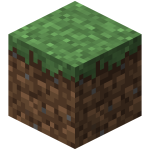
\includegraphics[width=0.15\textwidth]{graphics/block}
  \end{center}
  \caption{A~"Grass"~Block~\cite{image_mob}}
  \label{mc_block}
\end{wrapfigure}

In this section basic concepts of the game are described (in regards to our A.I. interface). Minecraft worlds are build out of blocks~(see figure ~\ref{mc_block}). Blocks are cubes. There are different types (materials) of blocks and they share a single size, which converts to the basic distance unit of Minecraft. One unit can be thought of as roughly equaling one meter.

\begin{wrapfigure}{l}{0.15\textwidth}
  \begin{center}
    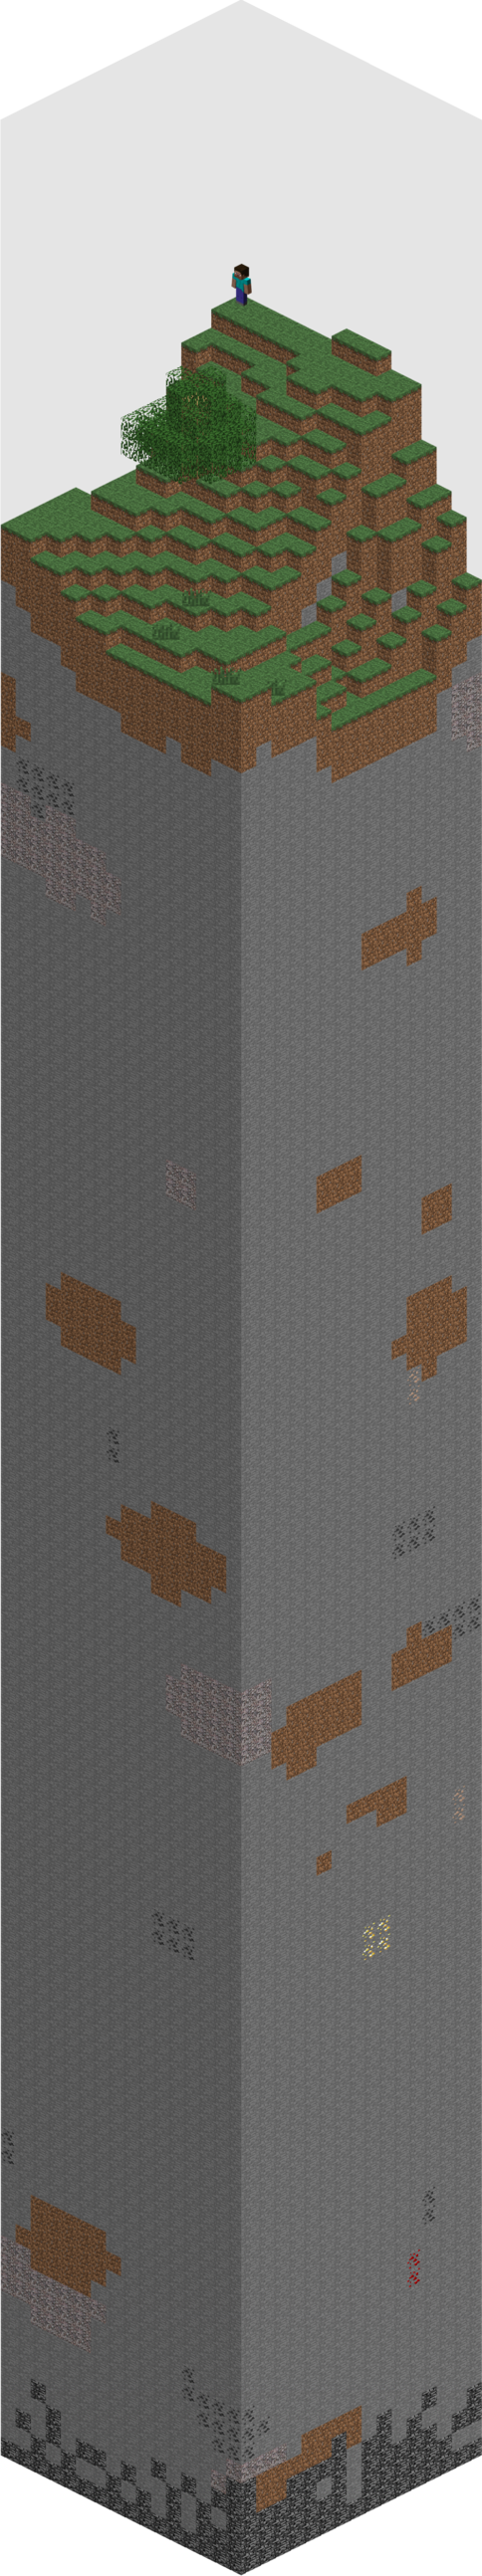
\includegraphics[width=0.04\textwidth]{graphics/chunk}
  \end{center}
  \caption{A~Chunk~\cite{image_mob}}
  \label{mc_chunk}
\end{wrapfigure}  

A chunk~(see figure ~\ref{mc_chunk}) is a segment of the Minecraft world that is 16 blocks long, 16 blocks wide and 256 blocks high (or deep) and therefore consists of up to 65,536 blocks.~\cite{mcwiki_chunks}

\begin{wrapfigure}{r}{0.3\textwidth}
  \begin{center}
    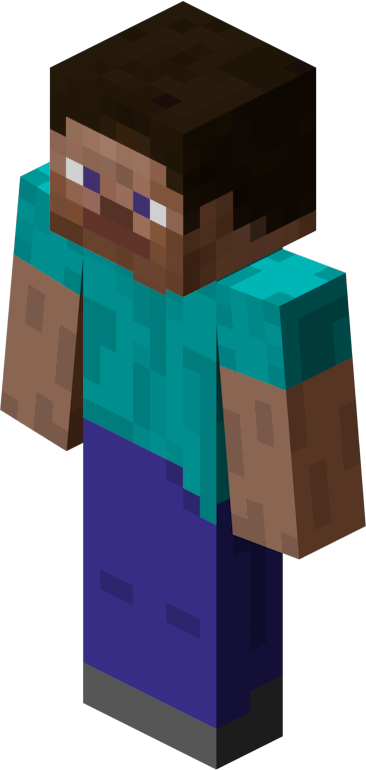
\includegraphics[width=0.08\textwidth]{graphics/player}
  \end{center}
  \caption{"The~Player"~\cite{image_mob}}
  \label{mc_player}
\end{wrapfigure} 

"The player"~(see figure ~\ref{mc_player}) is what the playable game-character in Minecraft is called. It is usually displayed humanoid.
Also, a Minecraft world has a day-night-cycle with 24 Minecraft hours converting to 14 minutes by default

The game itself has no predefined goals. Players can walk around, discover the generated world (see figure \ref{mc_mechanics} 1) and collect resources by ``destroying'' blocks , with the generated resources equaling the block type. They can combine different resources to ``craft'' items. For example, a player can destroy the blocks that represent a tree~(2). The gained ``wood'' resource could then be used to craft a wooden pickaxe~(2), which could then be used to dig into the ground more effectively~(4) to ``mine'' more rare resources, like iron or gold.

\begin{figure}[h]
  \centering
    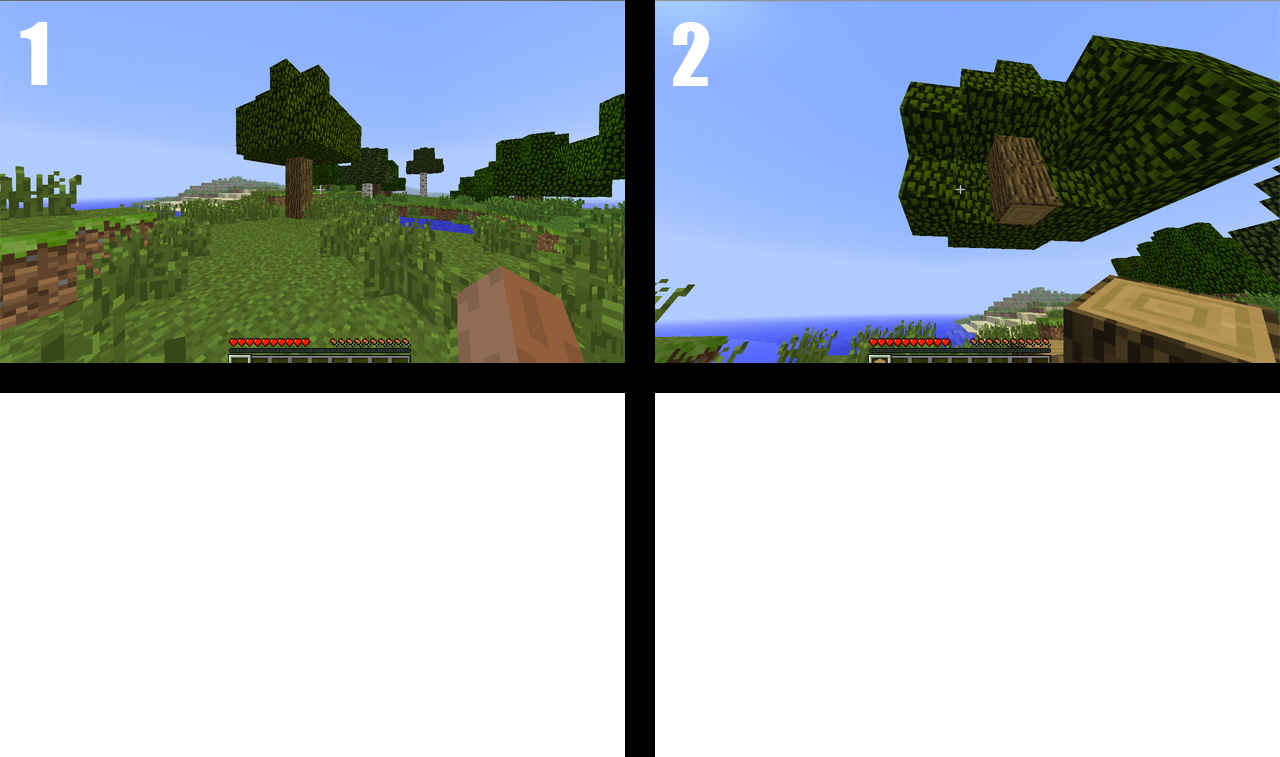
\includegraphics[width=15cm]{graphics/minecraft_mechanics}
  \caption{Minecraft Basic Mechanics  (CC-BY-3.0 Mojang AB)} %TODO find out copyright
  \label{mc_mechanics}
\end{figure}

There exist different game modes. The original "survival" mode adds monsters that attack the player at night. What solutions to survive the player comes up with (eg. building shelter or fighting the monsters) is left up to him or her.

In "creative" mode, the player is not being attacked by monsters, has the ability to fly and instant access to unlimited resources.

The mode of a Minecraft world does not effect the functionality of this project.

        \section{The Client Server Protocol}
Minecraft's Client-Server-Protocol is not publicly documented by the developers themselves. However, the modding-community gathered full knowledge and understanding of its structure (probably by using reverse engineering techniques). The protocol is based on packets. 

%TODO mention NBT file format

Packets are either "server to client", "client to server" or "Two-Way" and begin with a "Packet ID" byte. The structure of the packet's payload depends on it's Packet ID.
 
To give an example of one of the easier packets, the "Client Position"-Packet is fairly straight-forward~(see figure \ref{mc_packet}). It is exclusively send from clients to servers and starts with it's Packet ID (as every packet does), followed by the X- and Y-coordinates as doubles, the stance value as a double, which is used to to modify the player's bounding box, another double for the Z-coordinate and eventually a boolean that describes if the player is on the ground or not.~\cite{protocol}

\begin{table}[htb]
\centering
\begin{tabular}{|c|c|c|}\hline

    Field Name & Field Type & Notes \\ \hline
   Packet ID & Byte & 0x0B \\ \hline
   X & double & Absolute position \\ \hline
   Y & double & Absolute position \\ \hline
   Stance & double & Used to modify the players bounding box \\ \hline
   Z & double & Absolute position \\ \hline
   On Ground & boolean & Derived from packet 0x0A \\ \hline
   
\end{tabular}
\caption{Structure of the packet ``Player Position (0x0B)''~\cite{protocol}}
\label{mc_packet}
\end{table}

Knowledge of this data structure is already sufficient to move around in the Minecraft world. To go forward, one has to figure out the players current position, calculate the absolute coordinates of the destination of the movement in regard of it and send a Client Position packet with these coordinates to the server. If the destination is not more than 100 blocks away from the origin of the movement, the server accepts the packet. In the official Minecraft client, a players movement from one point to the other is rendered with a walking animation.

Other than movement, packet structures are defined for every aspect of the game. May it be the initial handshake, the creation or destruction of blocks or activities of other player- or non-player-characters.

This protocol is what a custom Minecraft client needs to speak.

        \section{Suitability of Minecraft as a simulation environment}
There are a number of reasons why using Minecraft as a simulation environment could be useful and lead to interesting results.

First, the game itself is easily accessible. It is developed using Java (for both the client and the server software) and therefore, up to a certain extend ,platform independent. The "desktop computer version" is being sold for Windows, Mac OS X and Linux devices. There are official ports for Android, iOS, Xbox 360, the Raspberry Pi and a version for the upcoming game console Xbox One is announced. The desktop versions are priced at 19.95 euros, which makes it affordable to a large audience.
%TODO find out how to typeset €

The game itself already has an enormous fanbase. It is (like most videogames) especially popular among teenagers. Minecraft being loved by so many people could benefit this project, in terms of leading to increased attention.

The game's developer has proven many times that it acts generously towards  other developers, when it comes to the creation of game modifications and content that uses, or changes original Minecraft intellectual property. In other words: Mojang is not restrictive towards users doing all kinds of things with their creations. This led to the availability of a fairly complete community-sourced  documentation and explanation of virtually every aspect of the game --- including it's software architecture, data structure and protocols. This is useful for this project, as chances are low that they will have anything against using Minecraft for this project in the foreseeable future. %(In fact, the game's A.I. creator Jon Kagström seems to be fond of this project)

The Minecraft world with it's logic, semantic and functionalities offers possibilities for an A.I. to prove being able to interact with the environment --- in primitive ways (e.g. moving around), as well as with increasingly complex tasks like building, collecting resources, crafting items and interacting appropriately with both well-disposed and hostile other entities.

The semantics of the gameworld share characteristics with the real world. Moving through a Minecraft environment, one quickly realises that the game has generated different biomes (eg. forest or tundra). Also, trees, rivers, mountains and ore veins are neither hard-coded, nor appear completely randomly, but are generated procedurally and their structure appears to be (somewhat) fractal.
        
Using Minecraft as a simulation environment will give Psi agents possibilities to show off, what kind of sophisticated behaviour they are capable of.

\section{Related Projects}
    \subsection{Minecraft Bots}
There exist many projects , that could be considered Minecraft ``bots''. One has to differentiate in between two types. On the one hand there are those, that mimic an entire client software and facilitate communication with the server on the default client software's behalf. On the other hand there are bots which are modifications of the original client (or server) software and usually add non player characters --- like animals and other non-human creatures --- to the game. The code is usually injected through one of the popular ``modloaders'' (eg. Minecraft Forge).

One example (and probably the most advanced one), for an entire bot framework that replaces the client, is Mineflayer.~\cite{github_mineflayer} It has a high-level abstraction of the environment (eg. entity knowledge and tracking) and is written in JavaScript using node.js. However, it has not been used for this project, because a Python implementation was aimed for.

Opposed to Mineflayer, an example for ``game modification'' bots are the ``Cubebots'' --- fan-made non-player characters that aim to help Minecraft players with mundane tasks.\cite{mcforums_cubebot}

    \subsubsection{\texttt{Spock} by Nick Gamberini}
Developed by Nick Gamberini, \texttt{Spock} is an open-source bot framework (and as such also a Minecraft client) written in Python. It has been chosen to become an essential part of this project for two reasons: being written in Python it painlessly integrates in the existing MicroPsi code and the absence of dependencies (with one exception) leave the code understandable and easy to deploy.
    
    \subsubsection{Protocol Implementation in \texttt{Spock}}
The Minecraft protocol implementation in \texttt{Spock} is straight-forward~(see figure\ref{snippet_structures}). The necessary data structures are stored separately and can be accessed globally.

		
		\begin{figure}[ht]
			\centering
			\begin{minipage}{11cm}
				\begin{pseudocode}
names = {
	0x00: "Keep Alive",
	0x01: "Login Request",
	0x02: "Handshake",
	0x03: "Chat Message",
	...

structs = {
	#Keep-alive
	0x00: ("int", "value"),
	#Login request
	0x01: (
			("int", "entity_id"),
			("string", "level_type"),
			("byte", "game_mode"),
			("byte", "dimension"),
			("byte", "difficulty"),
			("byte", "not_used"),
			("ubyte", "max_players")),
	...
					\end{pseudocode}
				\caption{data structures for the packet IDs and structures}
				\label{snippet_structures}
			\end{minipage}
		\end{figure}
		
The structures are used to parse each packet appropriately~(see figure \ref{snippet_parse}).

		\begin{figure}[ht]
			\centering
			\begin{minipage}{13cm}
				\begin{pseudocode}
	def decode(self, bbuff):
		#Ident
		self.ident = datautils.unpack(bbuff, 'ubyte')
		
		#print hex(self.ident)
		
		#Payload
		for dtype, name in mcdata.structs[self.ident][self.direction]:
			self.data[name] = datautils.unpack(bbuff, dtype)
					\end{pseudocode}
				\caption{function for decoding packets}
				\label{snippet_parse}
			\end{minipage}
		\end{figure}
		
		\subsection{Minecraft Clones}

Minecraft's success inspired many other projects - including a number of Minecraft-like games in a wide variety of programming languages and environments.

Interesting projects include Skycraft~\cite{skycraft}, a Minecraft-like browser-game based on WebGL.

A particular project, that has the same name as the original game that inspired it, is \texttt{Minecraft} by Michael Fogleman~(see figure~\ref{fogleman_mc_screen}). It is a simple Minecraft clone in under 600 lines of Python and gained some popularity on reddit~\cite{fogle-reddit} and Hacker News.~\cite{fogle_hn}

It is comparably easy to understand and modify and has been used for the visualisation component of this project. It is based on the Python multimedia library Pyglet~\cite{pyglet}.

\begin{figure}[h]
  \centering
    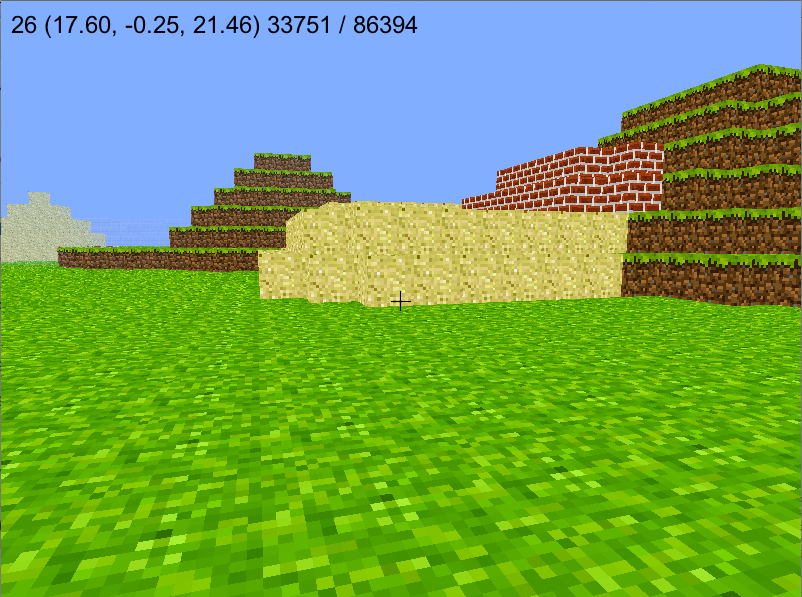
\includegraphics[width=10cm]{graphics/fogleman_mc_screen}
  \caption{\texttt{Minecraft} by Michael Fogleman}
  \label{fogleman_mc_screen}
\end{figure}
